\documentclass[titlepage, 11pt, letterpaper]{article}

% Packages
\usepackage[utf8]{inputenc}
\usepackage[margin=1in]{geometry}
\usepackage{csvsimple}
\usepackage{tabularx}
\usepackage{graphicx}
\usepackage{float}
\usepackage{multirow}
\usepackage{longtable}
\usepackage[utf8]{inputenc}
\usepackage[english]{babel}
\usepackage{nameref}
\makeatletter
\newcommand*{\currentsection}{\thesection \leftmark}
\newcommand*{\currentsubsection}{\thesubsection \leftmark}
\makeatother



\title{\Huge{Pollution Detection Network} \\ \vspace{0.5cm} \LARGE{Group 41}}
\author{
{
\centering
\begin{tabular}{c c}
Ian Wallace & Paul Wood  \\
\normalsize\textit{Computer Engineering} & \normalsize\textit{Computer Engineering} \\
& \\
Parke Benjamin & Randy Alvarez \\
\normalsize\textit{Electrical Engineering} & \normalsize\textit{Electrical Engineering} \\
\end{tabular}
}
}
\date{}

\usepackage{setspace}
\linespread{0.83}
\renewcommand{\arraystretch}{1.25}

% Requirement Counter
\newcounter{secRecNo}[section]
\newcounter{subSecReqNo}[subsection]



\begin{document}

\maketitle


\tableofcontents
\listoftables
\listoffigures
\newpage

\section{Introduction}
\subsection{Narrative Description and Motivation}
For this project, we plan to create a sensor network used for measuring quantities of certain pollutants over a certain area in an urban environment. The sensor network will consist of multiple identical nodes. These nodes will be physically mounted in various locations and evenly spread throughout the area to be monitored. Each node will contain various sensors that will be used to measure certain pollutants. Each node will also contain a LoRa transceiver that will be used to send the sensor data to a gateway. This gateway will process then send this data to an external server over the internet, where it can be further processed and analyzed. This network should help determine areas of concern with regards to pollution and, hopefully, allow for measures to be taken to reduce it.

\subsection{Project Goals}
\begin{itemize}
    \item The sensor nodes should be low cost. 
    \item The sensor nodes should be lightweight. 
    \item The sensor nodes should be able to read data in from the environment and that data through other nodes to the gateway. 
    \item The sensors nodes should be able to communicate over a large enough distance in order to make it feasible to cover large enough area with nodes.
    \item The nodes should require little to no maintenance.
    \item The sensor nodes should be easy to install.
    \item The gateway should be able to connect to the internet to send the data it receives from the nodes to an external server over the internet.
    
\end{itemize}

\section{Requirements and Constraints}
\subsection{Engineering Requirements}

\begin{table}[H]
\centering
\caption{The gateway requirements}
\begin{tabularx}{\linewidth}{|c|X|c|c|}
\hline
No. & Requirement & Value & Units \\
\hline\hline
1.0 & The gateway should cost no more than \$200 & 200 & dollars \\\hline
1.1 & The gateway should be no larger than 24" x 24" x 24" & 24x24x24 & inches \\\hline
1.2 & The gateway weight should be no more than than 10 pounds & 10 & lbs \\\hline
1.3 & The gateway should utilize LoRaWAN with the base station as the gateway with the capacity to connect with up to 8 devices simultaneously. & 8 & nodes \\\hline
1.4 & The gateway should be able to communicate with nodes up to 10 km away with ideal conditions & 10	& km \\\hline
1.5 & The gateway should be able to communicate with nodes up to 3 km away in an urban environment & 3 & km \\\hline
% & The gateway shall be able to connect to the Internet with at least a 512 Kbps upload/download link. & 512 & Kbps \\\hline
1.6 & The gateway should be able to manage up to 256 nodes & 256 & nodes \\\hline
% & The gateway shall configure the nodes such that the gateway can receive 256 node measurements per hour & 256 & measurements/hour \\\hline
\end{tabularx}
\label{tab:networkingRequirements}
\end{table}

\begin{table}[H]
\centering
\caption{The sensor node requirements.}
\begin{tabularx}{\linewidth}{|c|X|c|c|}
\hline
No. & Requirement & Value & Units \\
\hline\hline
2.0 & The sensor node should cost no more than \$150 & 150 & dollars \\\hline
2.1 & The sensor node should be no larger than 12" x 12" x 12" & 12x12x12 & inches \\\hline
2.2 & The sensor node weight should be no more than 10 pounds & 10 & lbs \\\hline
2.3 & The sensor node should stay operational without intervention for 1 year & 1 & year \\\hline
2.4 & The sensor node sensors should have a maximum tolerance of +/- 20\% & 20 & \% \\\hline
2.5 & The sensor node should transmit for no more than 30 seconds every 24 hours & 30 & seconds \\\hline

% & The sensor node PCB shall be no wider than TBD inches. & TBD & inches\\\hline
% & The sensor node shall stay in a low power state and draw less than 1 microamp when not reading from the sensor or transmitting data. & 1 & $\mu$A \\\hline
% & The nodes shall not consume more than 150 mW. & 150 & mW \\\hline
% & The nodes shall last one year before a battery replacement becomes necessary. & 1 & year \\\hline
% & The sensor node shall take a take a reading from the temperature sensor 1 time per hour. & 1 &reading/hour\\\hline
% & The sensor node shall take a take a reading from the O3 sensor 1 time per hour. & 1 & reading/hour\\\hline
% & The sensor node shall take a take a reading from the PM sensor 1 time per hour. & 1 & reading/hour\\\hline
% & The sensor node shall take a take a reading from the CO sensor 1 time per hour. & 1 & reading/hour\\\hline
% & The sensor node shall take a take a reading from the SO2 sensor 1 time per hour. & 1 & reading/hour\\\hline
% & The sensor node shall take a take a reading from the NO2 sensor 1 time per hour. & 1 & reading/hour\\\hline
% & The sensor node microcontroller shall draw no more than 50 mA when taking a sensor reading. & 50 & mA \\\hline
% & The sensor node microcontroller shall draw no more than 50 mA when transmitting data to the gateway. & 50 & mA\\\hline
% & The sensor node microcontroller shall have a clock speed of at least TBD MHz. & TBD & MHz\\\hline
% & The sensor node microcontroller shall have draw no more than 20 uA when waiting between switching to an active state. & 20 & microamp\\\hline
% & The sensor node shall have battery with at least 3000 mAH & 3000 & mAH\\\hline
% & The sensor node shall have a battery with a voltage of 3.3 V. & 3.3 & V\\\hline
\end{tabularx}
\label{tab:nodeRequirements}
\end{table}

\subsection{Engineering Specifications}
\begin{table}[H]
\centering
\caption{The gateway and networking engineering specifications}
\begin{tabularx}{\linewidth}{|c|X|}
\hline
No. & Requirement \\
\hline\hline
3.0 & The gateway shall use LoRa and LoRaWAN for the wireless communication protocol \\\hline
3.1 & The gateway should adhere to the LoRa Fair Access policy \\\hline
3.2 & The gateway should have enough internet bandwidth to support all of its connected nodes \\\hline
3.3 & The network shall utilize a star networking topology.\\\hline
3.4 & We define a component of our network to be known as a cell, which shall consist of nodes connected to a gateway. \\\hline
3.5 & The gateway shall be able communicate with an external server over the internet.\\\hline
3.6 & The server shall be hosted on existing web hosting platform.\\\hline
3.7 & The server shall host a website that displays data collected from the sensors.\\\hline
\end{tabularx}
\label{tab:networkingSpecs}
\end{table}

\begin{table}[H]
\centering
\caption{The node engineering specifications}
\begin{tabularx}{\linewidth}{|c|X|}
\hline
No. & Requirement \\
\hline\hline
4.0 & The sensor node shall use a radio and antenna that is part of a daughterboard that can be attached to the main PCB.\\\hline
4.1 & The node should use a battery and solar panel \\\hline
4.2 & The sensor node shall contain a microcontroller. \\\hline
4.3 & The sensor node microcontroller shall support the UART protocol.\\\hline
4.4 & The sensor node microcontroller shall have at least one ADC.\\\hline
4.5 & The sensor node microcontroller shall support JTAG debugging.\\\hline
4.6 & The sensor node shall contain a NO2 sensor.\\\hline
4.7 & The sensor node shall contain a PM sensor.\\\hline
4.8 & The sensor node shall contain a SO2 sensor.\\\hline
4.9 & The sensor node shall contain a O3 sensor.\\\hline
4.10 & The sensor node shall contain a CO sensor.\\\hline
\end{tabularx}
\label{tab:nodeSpecs}
\end{table}


\subsection{Constraints}
\begin{table}[H]
\centering
\caption{The constraints.}
\begin{tabularx}{\linewidth}{|X|}
\hline
Constraint \\
\hline
The nodes must be light enough so that they can be affixed to a building or other structure and not be of a concern to fall off.\\\hline
The nodes must low cost to be able to placed in greater number. \\\hline
The nodes must be able to withstand water from rainfall.\\\hline
The nodes must be able to withstand high winds. \\\hline
The nodes must be able to withstand temperature extremes. \\\hline
The nodes must be able to support a communication range of at least 1 km\\\hline
The nodes must be able to operate on less power than what one solar panel could generate in a single day to allow for operation when there is no sunlight present.\\\hline
The gateway must be able to operate off of mains power.\\\hline

\end{tabularx}
\label{tab:constraints}
\end{table}

\section{House of Quality}
\begin{figure}[H]
    \centering
    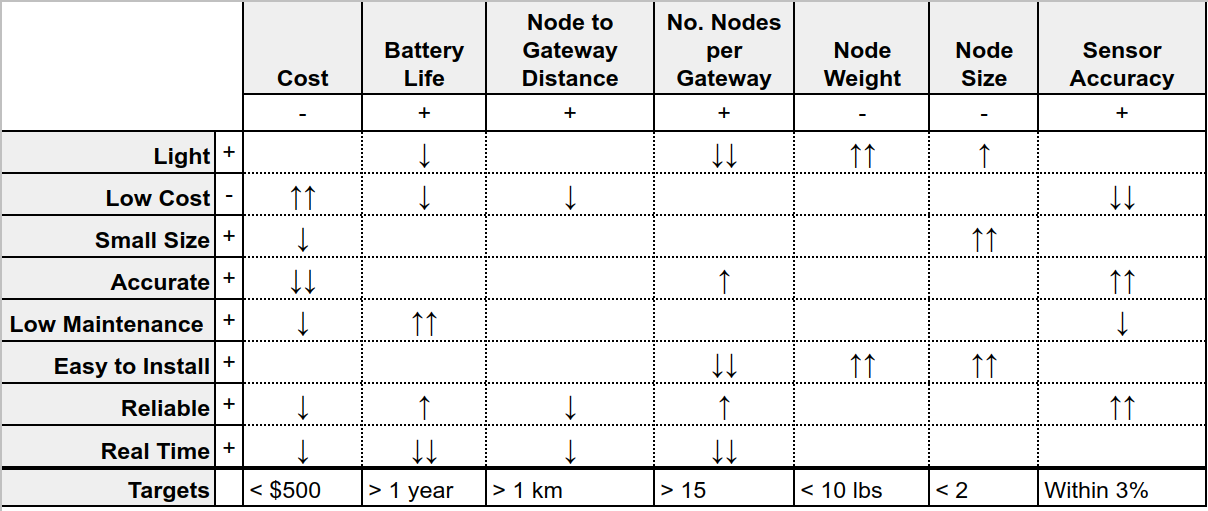
\includegraphics[width=6.25in]{"./hoq.png"} 
    \caption{The house of quality diagram.}
    \label{fig:hoq}
\end{figure}

\section{Stretch Goals}
\begin{tabularx}{\linewidth}{|X|c|c|}
\hline
Requirement & Value & Units \\
\hline
\hline

Operability with the decentralized Helium LoRa Network & Yes/No & Boolean \\\hline
% PSI and AQI forcasting N days in advance & N & days \\\hline
Increased sensor accuracy & 10-15 & percent \\\hline
Twitter alerts for hazardous air pollution & Yes/No & Boolean \\\hline
Increased battery life of the sensor nodes & 2-4 & years \\\hline
Sensor nodes are completely sustainable through the use of solar panels & Yes/No & Boolean \\\hline
Increased sensor node LoRa range in highly urban environments & 4-5 & km \\\hline
Highly responsive and modern graphical user interface (web site) & Yes/No & \\\hline

%  Support for sensors nodes to double as relay nodes for 1 hop 
\end{tabularx}


\section{Block Diagrams}

% Block Diagram for Node HW
\subsection{Sensor Node Hardware Diagram}
\begin{figure}[H]
    \centering
    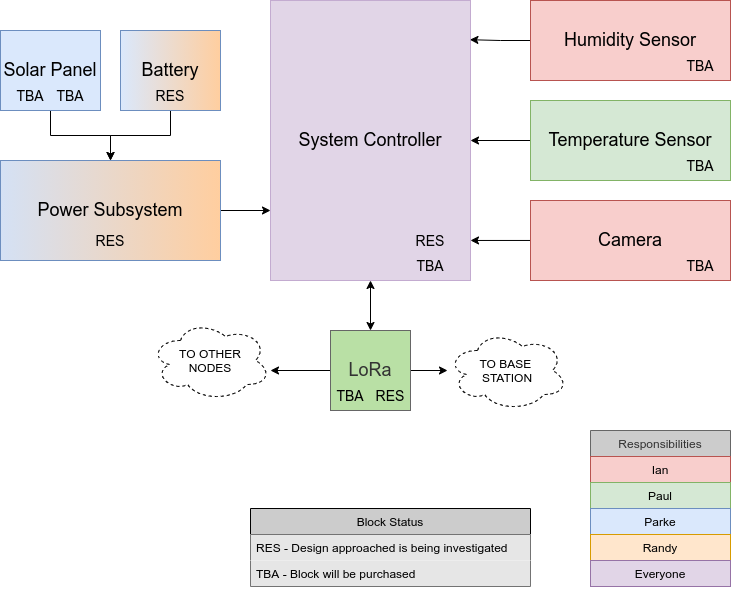
\includegraphics[width=3.25in]{"./hwNodeBD.png"} 
    \caption{The block diagram for the sensor node hardware.}
    \label{fig:hwNodeBD}
\end{figure}

% Block Diagram for gateway HW
\subsection{Gateway Hardware Diagram}
\begin{figure}[H]
    \centering
    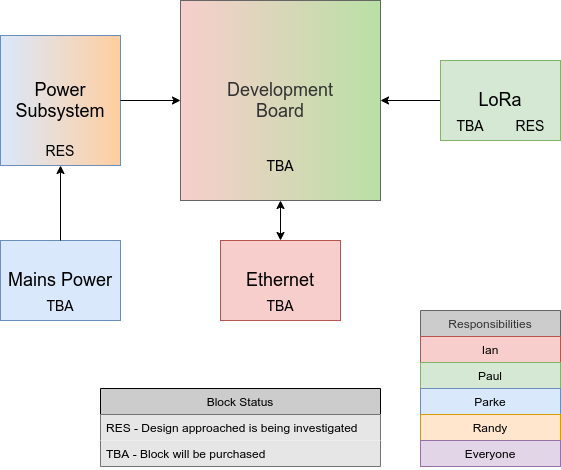
\includegraphics[width=3.25in]{"./hwGatewayBD.png"} 
    \caption{The block diagram for the gateway hardware.}
    \label{fig:hwBaseStationBD}
\end{figure}

% TODO: gateway software
% Block Diagram for Node SW
\subsection{Sensor Node Software Diagram}
\begin{figure}[H]
    \centering
    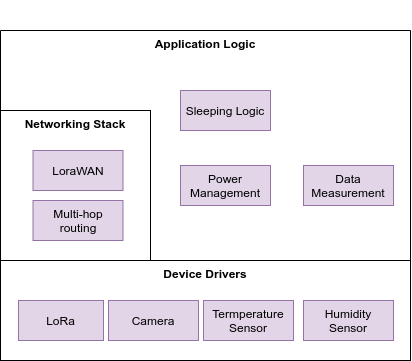
\includegraphics[width=4in]{"./swNodeBD.png"} 
    \caption{The block diagram for the node software.}
    \label{fig:swNodeBD}
\end{figure}

\begin{table}[H]
    \centering
    \caption{A description of each block in the sensor node hardware block diagram.}
    \begin{tabularx}{\linewidth}{|c|X|}
        \hline
        Block Name & Description \\ 
        \hline
        Battery & The battery will take in power from the power subsystem and will store whatever is left over from the consumption by the system controller. \\\hline
        Power Subsystem & The power subsystem will take in and regulate power from the solar panel charging the battery as well as taking power from the battery for whatever needs the system controller requires. The power subsystem will also invert the DC power from the solar panel and battery to AC if required. \\\hline
        Solar Panel & The solar panel will feed power to the power subsystem where a solar power controller will be placed to take in the generated power. \\\hline
        System Controller & The system controller take in and process data from the sensors and output data to the LoRa transceiver. \\\hline
        Temperature Sensor & The temperature sensor will take a measurement of the current temperature and send it to the system controller. \\\hline
        O$_3$ Sensor & The temperature sensor will take a measurement of the current amount of detected ozone (O$_3$) and send it to the system controller. \\\hline
        CO Sensor & The temperature sensor will take a measurement of the current amount of detected carbon monoxide (CO) and send it to the system controller. \\\hline
        SO$_2$ Sensor & The temperature sensor will take a measurement of the current amount of detected sulfur dioxide (SO$_2$) and send it to the system controller. \\\hline
        NO$_2$ Sensor & The temperature sensor will take a measurement of the current amount of detected nitrogen dioxide (NO$_2$) and send it to the system controller. \\\hline
        PM Sensor & The temperature sensor will take a measurement of the current amount of detected particulate matter (PM) and send it to the system controller. \\\hline
        LoRa & The LoRa transceiver will receive data from the system controller and send that data to the gateway. \\\hline
    \end{tabularx}
    
    \label{tab:descHWNodeBD}
\end{table}

\begin{table}[H]
    \centering
    \caption{A description of each block in the gateway hardware block diagram.}
    \begin{tabularx}{\linewidth}{|c|X|}
        \hline
        Block Name & Description \\ 
        \hline
        Power Subsystem & The power subsystem will take in power from the battery for whatever needs the development board requires. The power subsystem will also invert the DC power from the solar panel and battery to AC if required. \\\hline
        Mains Power & This is the AC power coming from a wall outlet. \\\hline
        Ethernet & The Ethernet module will allow the development board to connect to the internet. \\\hline
        LoRa & The LoRa transceiver will receive data from the sensor nodes and send that data to the development board. \\\hline
        Development Board & The development board will process the sensor data received from the sensor nodes. This data will then be sent to an external server over the internet where it can be analyzed. \\\hline
    \end{tabularx}
    \label{tab:descHWBaseStationBD}
\end{table}

\begin{table}[]
    \centering
    \caption{A description of each block in the sensor node software block diagram.}
    \begin{tabularx}{\linewidth}{|c|X|}
        \hline
        Block Name & Description \\ 
        \hline
        Power Management & This software will responsible for controlling and monitoring the power subsystem.  \\\hline
        Data Management & This software will be responsible for processing data received from the sensors. \\\hline
        Sleeping Logic & This software will handle the logic for switching between taking sensor measurements and residing in a low-power "sleep" mode between sensor measurements. \\\hline
        LoRa & This is a device driver for the LoRa transceiver. \\\hline
        Temperature Sensor & This is a device driver for the temperature sensor. \\\hline
        O$_3$ Sensor & This is a device driver for the O$_3$ sensor. \\\hline
        CO Sensor & This is a device driver for the CO sensor. \\\hline
        SO$_2$ Sensor & This is a device driver for the SO$_2$ sensor. \\\hline
        NO$_2$ Sensor & This is a device driver for the NO$_2$ sensor. \\\hline
        PM Sensor Sensor & This is a device driver for the PM sensor. \\\hline
        LoRaWAN & This handles the networking for the LoRa networking. \\\hline
        Multi-hop Routing & This software will control how traffic is routed around the sensor node network. \\\hline
    \end{tabularx}
    \label{tab:descSWNodeBD}
\end{table}

\section{Estimated Budget}
\begin{table}[H]
\centering
    \begin{tabular}{|c|c|c|l|}
        \hline
        Component & Unit Cost & Quantity & Total Cost \\
        \hline\hline
        Solar Panel                 & \$30.00 & 1 & \$30.00 \\
        Solar Charge Regulator      & \$5.00 & 1 & \$5.00 \\
        Battery                     & \$10.00 & 1 & \$10.00 \\
        Electronic Components       & \$10.00 & 1 & \$10.00 \\
        \hline
        LoRa Transceiver            & \$30.00 & 1 & \$30.00 \\
        Microcontroller             & \$3.00  & 1 & \$3.00  \\
        PCB                         & \$10.00 & 1 & \$10.00 \\
        Electronic Components       & \$10.00 & 1 & \$10.00 \\
        \hline
        O$_3$ Sensor                & \$49.00 & 1 & \$49.00\\
        Temperature Sensor          & \$4.00  & 1 & \$8.00 \\
        CO Sensor                   & \$20.00 & 1 & \$20.00\\
        SO$_2$ Sensor               & \$90.00 & 1 & \$90.00\\
        NO$_2$ Sensor               & \$50.00 & 1 & \$50.00\\
        PM Sensor               & \$50.00 & 1 & \$50.00\\
        \hline\hline
        \multicolumn{2}{|}{Multirow} & Total & \$371.00 \\
        \hline
    \end{tabular}
    \caption{The budget for each node.}
\end{table}

\begin{table}[H]
\centering
    \begin{tabular}{|c|c|c|c|}
        \hline
        Component & Approx. Unit Cost & Quantity & Total Cost \\
        \hline\hline
        Power Subsystem Components  & \$10.00 & 1 & \$10.00 \\
        \hline
        LoRa Transceiver            & \$40.00 & 1 & \$40.00 \\
        Antenna                     & \$40.00 & 1 & \$40.00 \\
        Raspberry Pi 4              & \$35.00 & 1 & \$35.00   \\
        Electronic Components       & \$10.00 & 1 & \$10.00 \\
        \hline\hline
        \multicolumn{2}{|}{Multirow} & Total & \$135 \\
        \hline
    \end{tabular}
    \caption{The budget for the gateway.} 
\end{table}


\section{Milestones}

\subsection{Fall Semester}
% TODO: Change spacing of the columns to make the description wider
%%%%%%%%%%%%%%%%%%%%%%%%%%%%%%%%%%%%%%%%%%%%%%%%%%%%%%%%%%%%%%%%
%
%                       Fall Milestones
%
%%%%%%%%%%%%%%%%%%%%%%%%%%%%%%%%%%%%%%%%%%%%%%%%%%%%%%%%%%%%%%%%
\begin{table}[H]
    \begin{tabularx}{\linewidth}{|c|X|X|}
        \hline
        Date & Milestone & Deliverables \\
        \hline\hline
        Sep. 2nd, 2021 
        & Sensing mechanism finalized 
        & Sensor requirements document \\
        
        \hline
        Oct. 1st, 2021
        & MCU and LoRa module finalized
        & Order confirmation and, if available, shipment information. \\
        
        \hline
        Oct. 8th, 2021 
        & Sensors finalized 
        & Order confirmation and, if available, shipment information. \\
        
        \hline
        Nov. 5th, 2021 
        & Software alpha 1.0 
        & Software alpha 1.0 node and base-station release binaries. \\ 
        
        \hline
        Nov. 19th, 2021 & Prototype v1.0 PCB 
        & PCB masks, fab order confirmation and, if available, shipment information \\
        
        \hline
        Dec 3rd, 2021 & Prototype v1.5 PCB 
        & PCB masks, fab order confirmation and, if available, shipment information \\
        
        \hline
        Dec 10th, 2021 
        & Software alpha 1.5 
        & Software alpha 1.5 node and base-station release binaries. \\ 
        
        \hline
    \end{tabularx}
    \caption{Fall milestones}
\end{table}

%%%%%%%%%%%%%%%%%%%%%%%%%%%%%%%%%%%%%%%%%%%%%%%%%%%%%%%%%%%%%%%%
%
%                   Fall Milestones Descriptions
%
%%%%%%%%%%%%%%%%%%%%%%%%%%%%%%%%%%%%%%%%%%%%%%%%%%%%%%%%%%%%%%%%
\begin{table}[H]
    \centering
    \begin{tabularx}{\linewidth}{|c|X|}
        \hline
        Project Milestone & Description 
        \\
        \hline\hline
        Sensing mechanism finalized &
        Finish research and create design requirements for accurately detecting wildfires in a cost effective way.
        \\
        
        
        \hline
        MCU and LoRa module finalized &
        The MCU, LoRa module/daughter-boards, and Raspberry Pi's are chosen, and multiple developer boards have been ordered to design and test mesh networking.
        \\
        
        \hline
        Sensors finalized 
        & The required sensors are chosen, and multiple parts/developer-boards have been ordered.
        \\
        
        \hline
        Software alpha 1.0 
        & The nodes can communicate and route packets to the gateway, and the gateway can communicate with all or specific nodes on the network. There also exists some sort of command line interface on the gateway to talk to the nodes, but there are no required internet capabilities of the base, yet. The nodes can go to sleep, but a sleep routine isn't configured optimally.
        \\
        
        \hline
        Prototype v1.0 PCB 
        & A PCB first version prototype PCB has been designed and ordered from a fast-turnaround PCB fab containing all required functionalities: power subsystem, MCU, LoRa module connectivity, battery and solar I/O, and sensor I/O with adequate noise isolation and filtering.
        \\
        
        \hline
        Prototype v1.5 PCB
        & PCB prototype with, if any, major issues fixed. Should also include sensor daughter boards.
        \\
        
        \hline
        Software alpha 1.5
        & The software works on the prototype PCB
        \\
        
        \hline
    \end{tabularx}
    \caption{Fall milestone descriptions}
\end{table}

\subsection{Spring Semester}
% TODO: Change spacing of the columns to make the description wider
%%%%%%%%%%%%%%%%%%%%%%%%%%%%%%%%%%%%%%%%%%%%%%%%%%%%%%%%%%%%%%%%
%
%                       Spring Milestones
%
%%%%%%%%%%%%%%%%%%%%%%%%%%%%%%%%%%%%%%%%%%%%%%%%%%%%%%%%%%%%%%%%
\begin{table}[H]
    \begin{tabularx}{\linewidth}{|X|X|X|}
        \hline
        Date & Milestone & Deliverables \\
        \hline\hline
        Jan. 19th, 2022 
        & Prototype v2.0 PCB 
        & PCB masks, fab order confirmation and, if available, shipment information \\
        
        \hline
        Jan. 19th, 2022
        & Enclosure prototype
        & Model and 3D printed enclosure
        \\
        
        \hline
        Jan. 29th, 2022 
        & Software alpha 2.0 
        & Software alpha 2.0 node and base-station release binaries
        \\
        
        \hline
        Feb. 18th, 2022
        & REST API created
        & REST API documentation and testing/validation scripts
        \\
        
        \hline
        Feb. 18th, 2022
        & Enclosure finalized
        & Model and 3D printed enclosure
        \\
        
        \hline
        Feb. 25th, 2022
        & Final v1.0 PCB
        & PCB masks, fab order confirmation and, if available, shipment information 
        \\
        
        \hline
        Mar. 1st, 2022
        & Software release v1.0
        & Software v1.0 node and base-station release binaries. 
        \\ 
        
        \hline
        Mar. 18st, 2022
        & Software release v1.1
        & Software v1.1 node and base-station release binaries. 
        \\ 
        
        \hline
        Mar. 18st, 2022
        & Final v1.1 PCB
        & PCB masks, fab order confirmation and, if available, shipment information 
        \\
        
        \hline
        Mar. 25th, 2022
        & Simple website to visualize results
        & Website front-end and back-end files, and website URL or IP
        \\
        
        % stretch goal
        %\hline
        %Mar. 25th, 2022
        %& Twitter integration
        %& Twitter account
        %\\
        
        \hline
    \end{tabularx}
    \caption{Spring milestones}
\end{table}
%%%%%%%%%%%%%%%%%%%%%%%%%%%%%%%%%%%%%%%%%%%%%%%%%%%%%%%%%%%%%%%%
%
%                   Spring Milestones Descriptions
%
%%%%%%%%%%%%%%%%%%%%%%%%%%%%%%%%%%%%%%%%%%%%%%%%%%%%%%%%%%%%%%%%
\begin{table}[H]    
    \centering
    \begin{tabularx}{\linewidth}{|c|X|}
        \hline
        Project Milestone & Description 
        \\
        \hline\hline
        Prototype v2.0 PCB 
        & This version should fix most or all remaining hardware bugs, and ensure accurate sensor readings. It should also be mountable in an enclosure.
        \\
        
        \hline
        Enclosure prototype
        & An enclosure O-rings, or some other kind of sealant, to keep out dust and water splashes. It should be able to mount the sensors to get environmental readings, and provide space for top-mounted solar-panel.
        \\
        
        \hline
        Software alpha 2.0 
        & The gateway should be able to set the node's sleep routine settings, and schedule any specific times to wake up at. The command-line utility should be robust enough with minimal bugs.
        \\
        
        \hline
        REST API created
        & The gateway should run a server and/or relay to bigger server to provide a REST API for clients to query data about environmental readings pertaining to wildfires.
        \\
        
        \hline
        Enclosure finalized
        & The enclosure that can house a PCB and mostly not get wet should be good enough.
        \\
        
        \hline
        Final v1.0 PCB
        & A PCB should be bug-free, and sent to a proper fab to have high-quality board material and a water resistant coating.
        \\
        
        \hline
        Software release v1.0
        & The software should be able to handle errors gracefully, reliably establish connections on the mesh network, and reliably wake-up and transmit data.
        \\ 
        
        \hline
        Software release v1.1
        & Bug fixes and minor improvements.
        \\ 
        
        \hline
        Final v1.1 PCB
        & Only if needed. Bug fixes and minor improvements.
        \\
        
        \hline
        Simple website to visualize results
        & The website doesn't need to look pretty, but it should provide a nice visualization of the nodes deployed plus data readings over time displayed in a graph.
        \\
        
        \hline
    \end{tabularx}
    \caption{Spring milestone descriptions}
\end{table}

\section{Decision Matrix}

\begin{table}[H]
    \centering
    
    \begin{tabularx}{\linewidth}{|c|X|X|X|}
        \hline
        Project Idea Name & Cost & Practicality & Familiarity \\
        \hline
        Forest Fire Sensor Network &
        Large number of nodes may lead to higher cost. Required sensors (humidity, camera) are more expensive. &
        Difficult to verify functionality of design i.e. need way to replicate forest fire, may require setting up nodes in an actual forest &
        Team members not familiar with working with LoRa and complex networking \\\hline
        
        Smart Aeroponics System &
        Requires building only one system. Less expensive sensors. &
        Straightforward verification of functionality. Very centralized system. &
        Standard networking requirements (client/server model). \\\hline
        
        Smart Home Management System 
        & Requires lots of WiFi transceivers, along with bright RBG LEDs for light fixtures. Relatively inexpensive (I hope).
        & Straightforward verification, and provides utility after senior design
        & Standard networking requirements (client/server model).
        \\\hline
        
        Power Line Protection 
        & Requires a 300 and 2 400 series microprocessor relays as well as a varying amount of fiber optic cable which would be very expensive
        & This would combine the speed of a 400 line differential protection scheme with the utility of a step distance relay
        & Team members would have to learn about power line protection schemes to complete project
        \\\hline
        
    \end{tabularx}
    \caption{A decision matrix of potential project ideas.}
\end{table}

\begin{table}[H]
    \centering
    \begin{tabularx}{\linewidth}{|c|X|}
        \hline
        Project Idea Name & Description \\
        \hline
        Forest Fire Sensor Network &
        A network of sensor nodes designed to detect a forest fire early and alert the appropriate people before it can spread. \\\hline
        
        Smart Aeroponics System &
        This would be a smart aeroponics system that utilizes various sensors and data processing to grow plants. Would contain sensors such as moisture and light. Could be remotely monitored and controlled via a website/app. Could utilize machine learning to detect various potential plant issues. \\\hline
        
        Smart Home Management System 
        & Create a personalized smart-home experience where preferences are stored for each person in the house, and profiles are chosen based on the connect WiFi devices and/or facial detection when entering the door. Positions in the house can be tracked to automatically turn on lights where you walk, and to play music and set an ambiance when you get home.
        \\
        
        \hline
        Power Line Protection &
        Creating a new protection relay that combines the functionality of 2 other protection schemes. It combines line differential which requires fiber optic between 2 substations that allows the relays to detect and solve problems almost instantly. It also uses step distance which uses a mathematical formula to calculate the position of a power line fault giving field crews the ability to know exactly where a problem is on a power line as they come up. \\\hline
    
    \end{tabularx}
    \caption{A description of each project idea.}
\end{table}

\end{document}
